\begin{figure}
\center

\begin{comment}
python3 CounterfactualModel_Remington_VIZ_Components.py 2 0 10.0 400 1000 UNIFORM UNIMODAL2 4567

\end{comment}

%%%%%%%
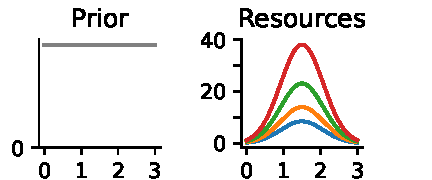
\includegraphics[width=0.35\textwidth]{figures/CounterfactualModel_Remington_VIZ_Components.py_4567_UNIFORM_UNIMODAL2_2_0_10.0_400.pdf}
%%%%%%%

  \begin{tabular}{@{}c@{}c@{}c@{}}
    % Row 1
    $p=0$ & $p=1$ & $p=2$ \\[-1.4ex]
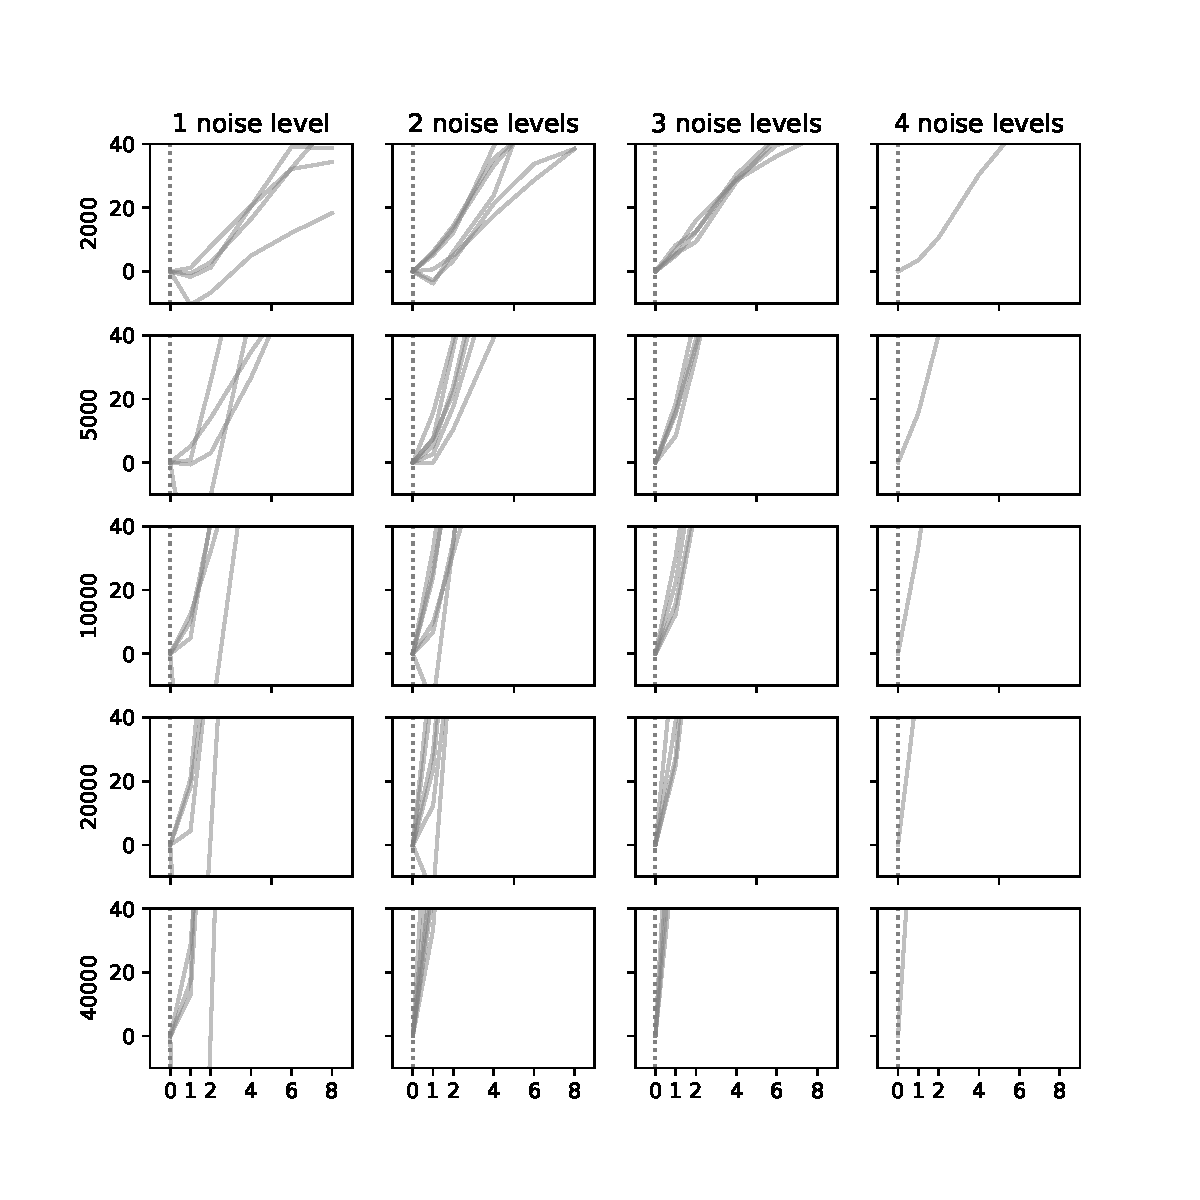
\includegraphics[width=0.33\textwidth]{figures/evaluateCrossValidationResults_Synthetic_Remington_VisualizeByNoiseCount_AndSize_ByP_Poster.py_UNIFORM_UNIMODAL2_0.pdf} &
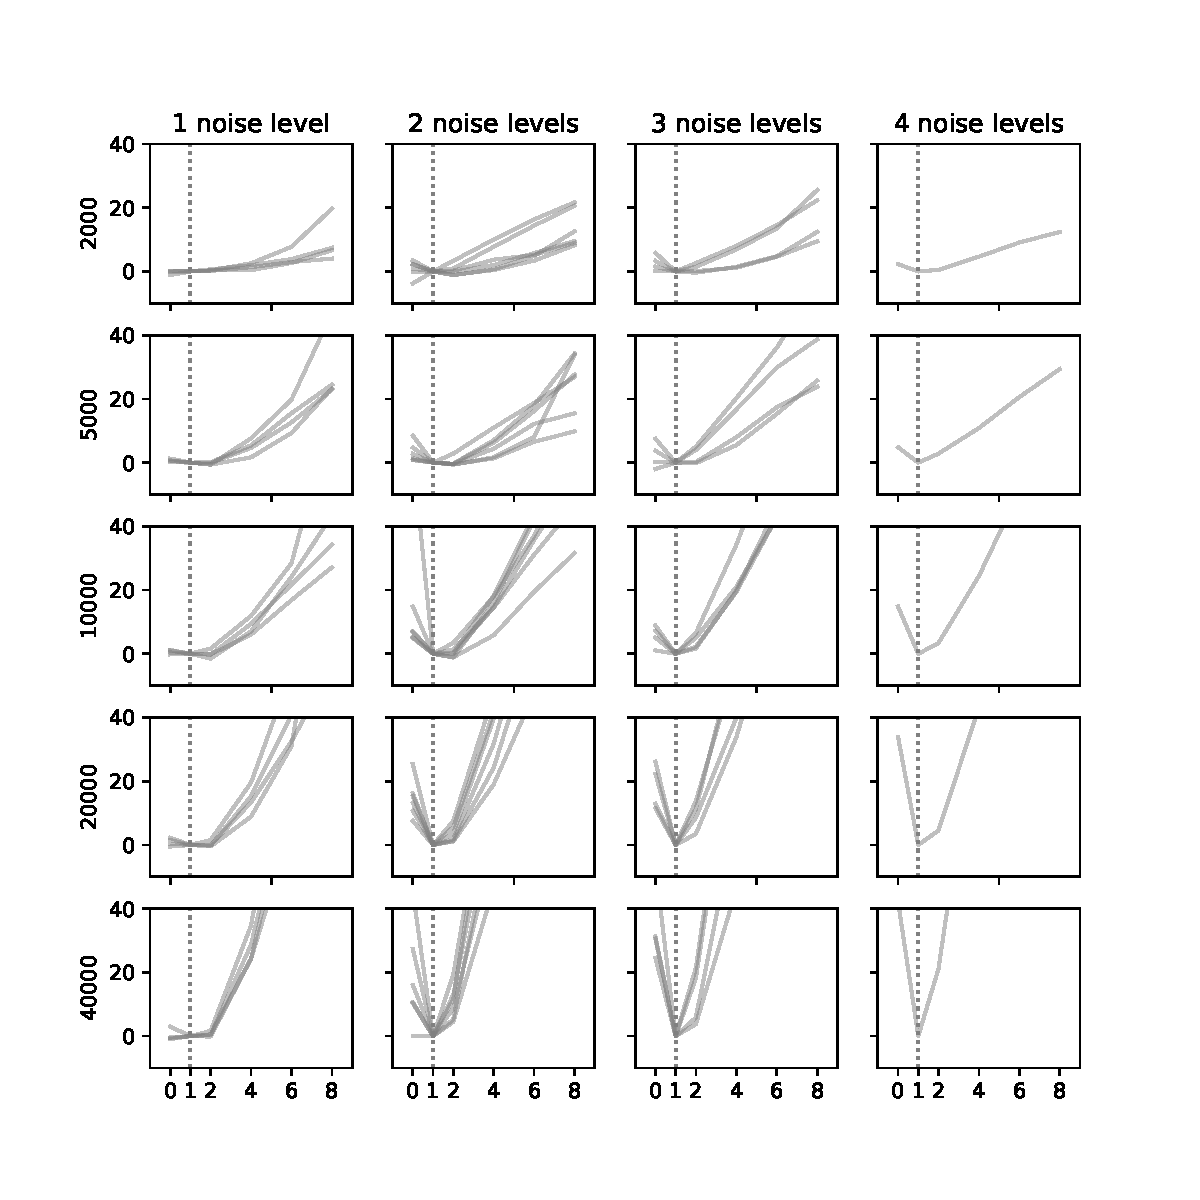
\includegraphics[width=0.33\textwidth]{figures/evaluateCrossValidationResults_Synthetic_Remington_VisualizeByNoiseCount_AndSize_ByP_Poster.py_UNIFORM_UNIMODAL2_1.pdf} &
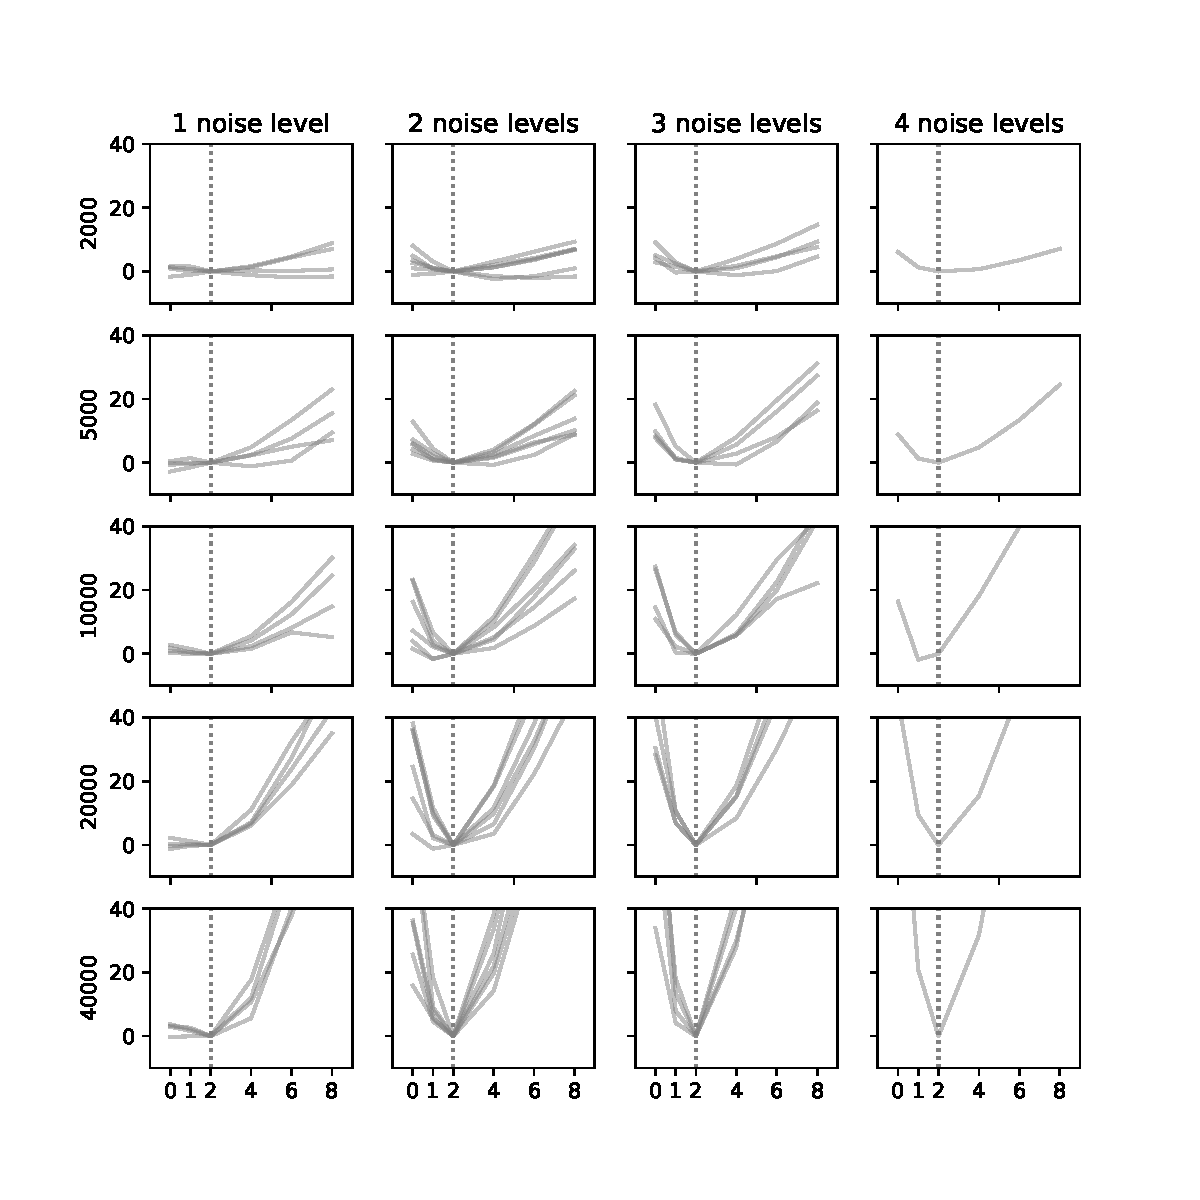
\includegraphics[width=0.33\textwidth]{figures/evaluateCrossValidationResults_Synthetic_Remington_VisualizeByNoiseCount_AndSize_ByP_Poster.py_UNIFORM_UNIMODAL2_2.pdf}  \\[-2ex]
$p=4$ &    $p=6$ & $p=8$ \\[-1.4ex]
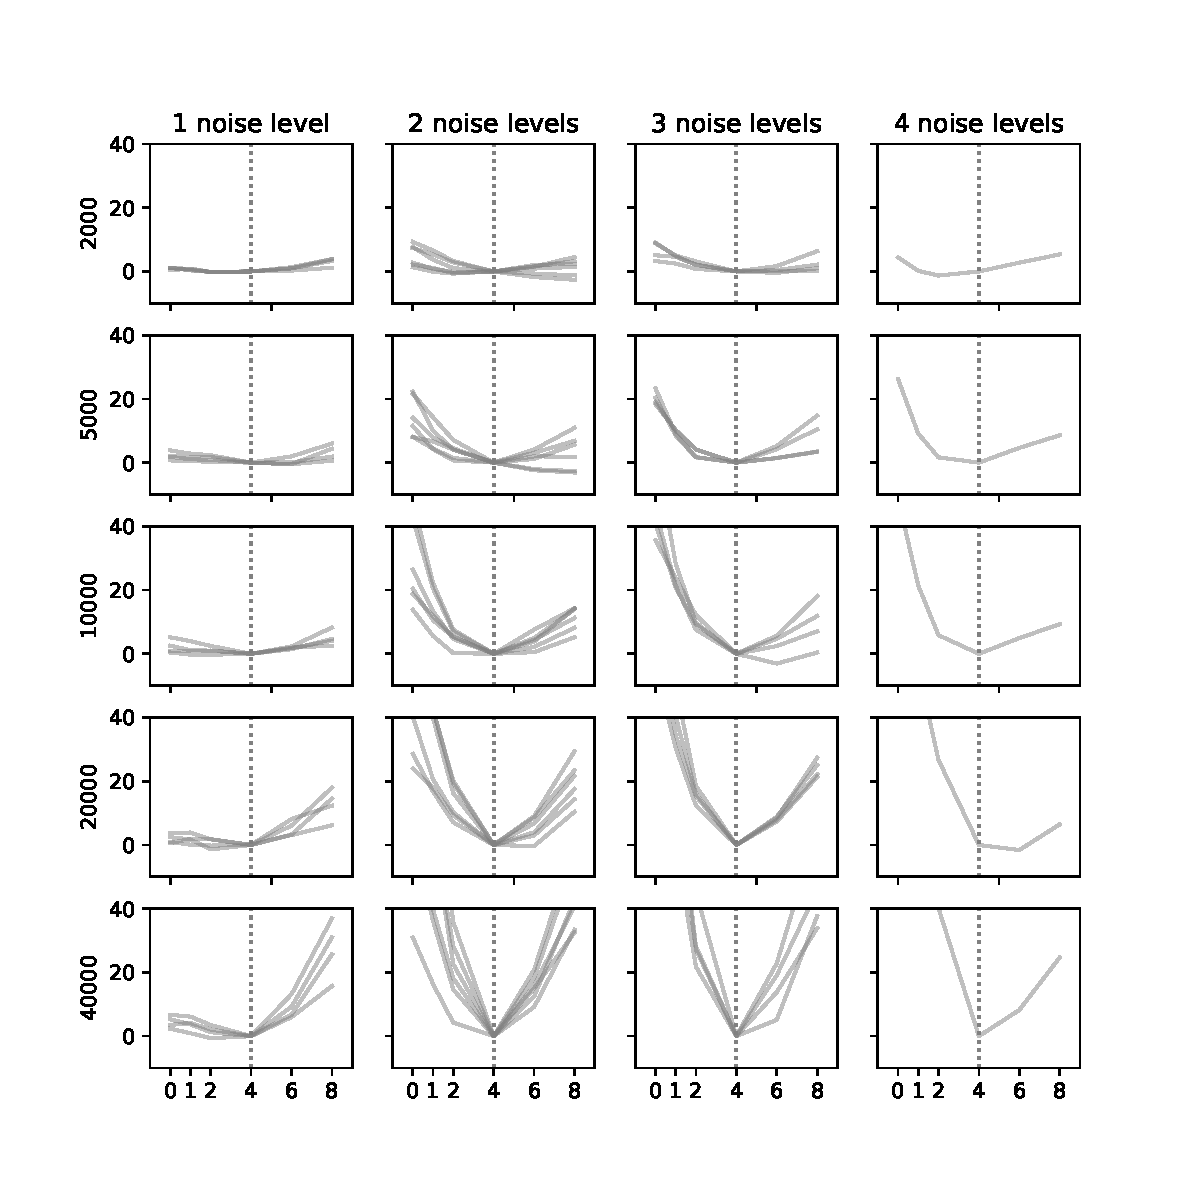
\includegraphics[width=0.33\textwidth]{figures/evaluateCrossValidationResults_Synthetic_Remington_VisualizeByNoiseCount_AndSize_ByP_Poster.py_UNIFORM_UNIMODAL2_4.pdf} &
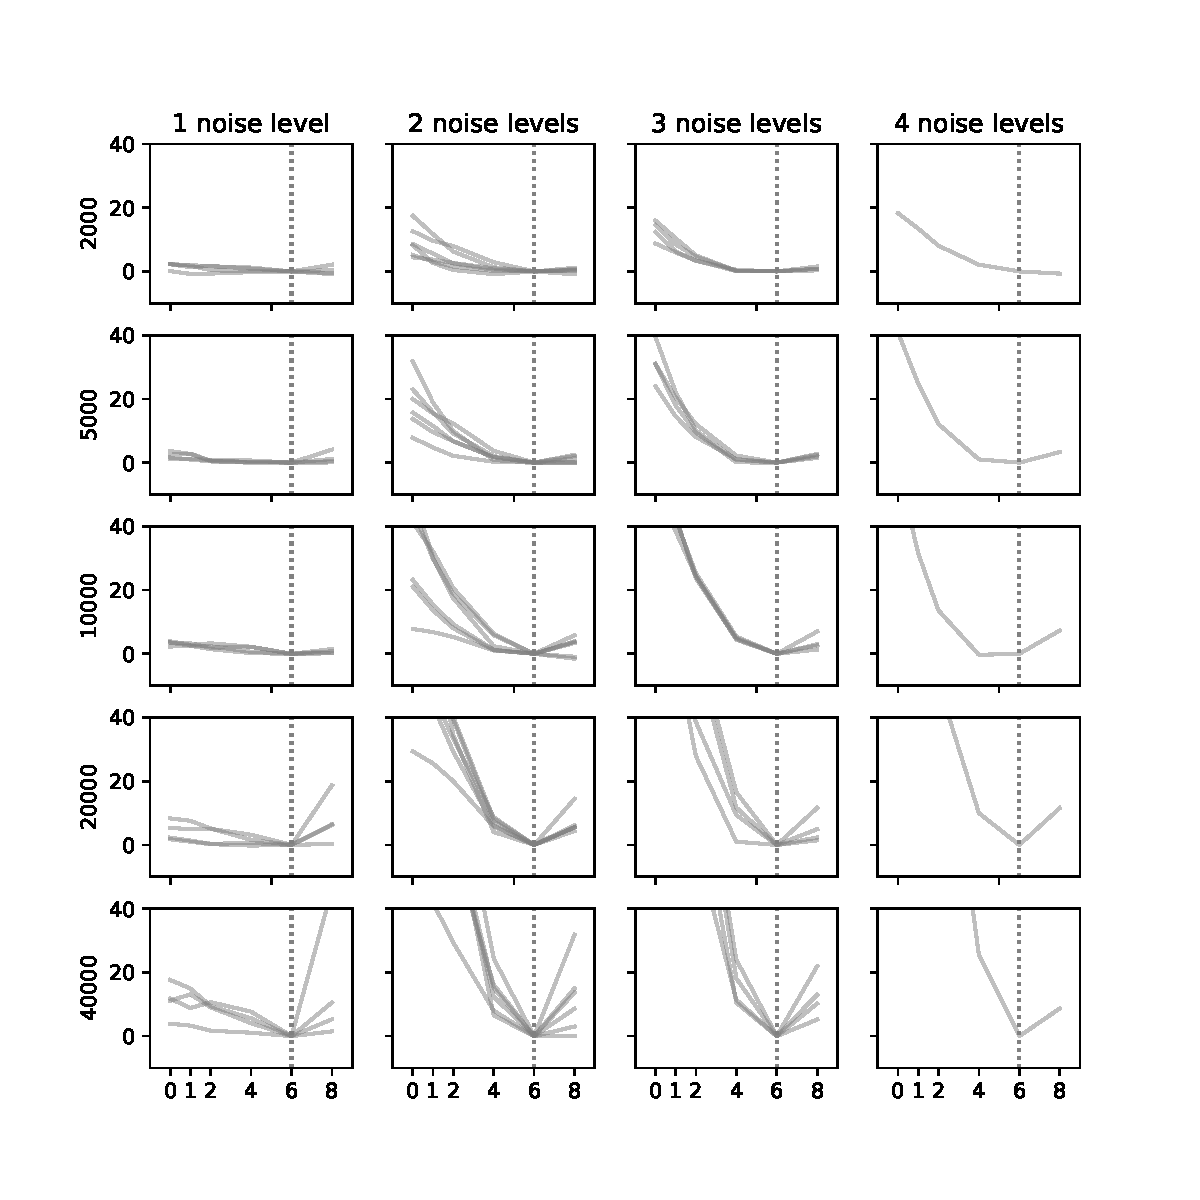
\includegraphics[width=0.33\textwidth]{figures/evaluateCrossValidationResults_Synthetic_Remington_VisualizeByNoiseCount_AndSize_ByP_Poster.py_UNIFORM_UNIMODAL2_6.pdf} &
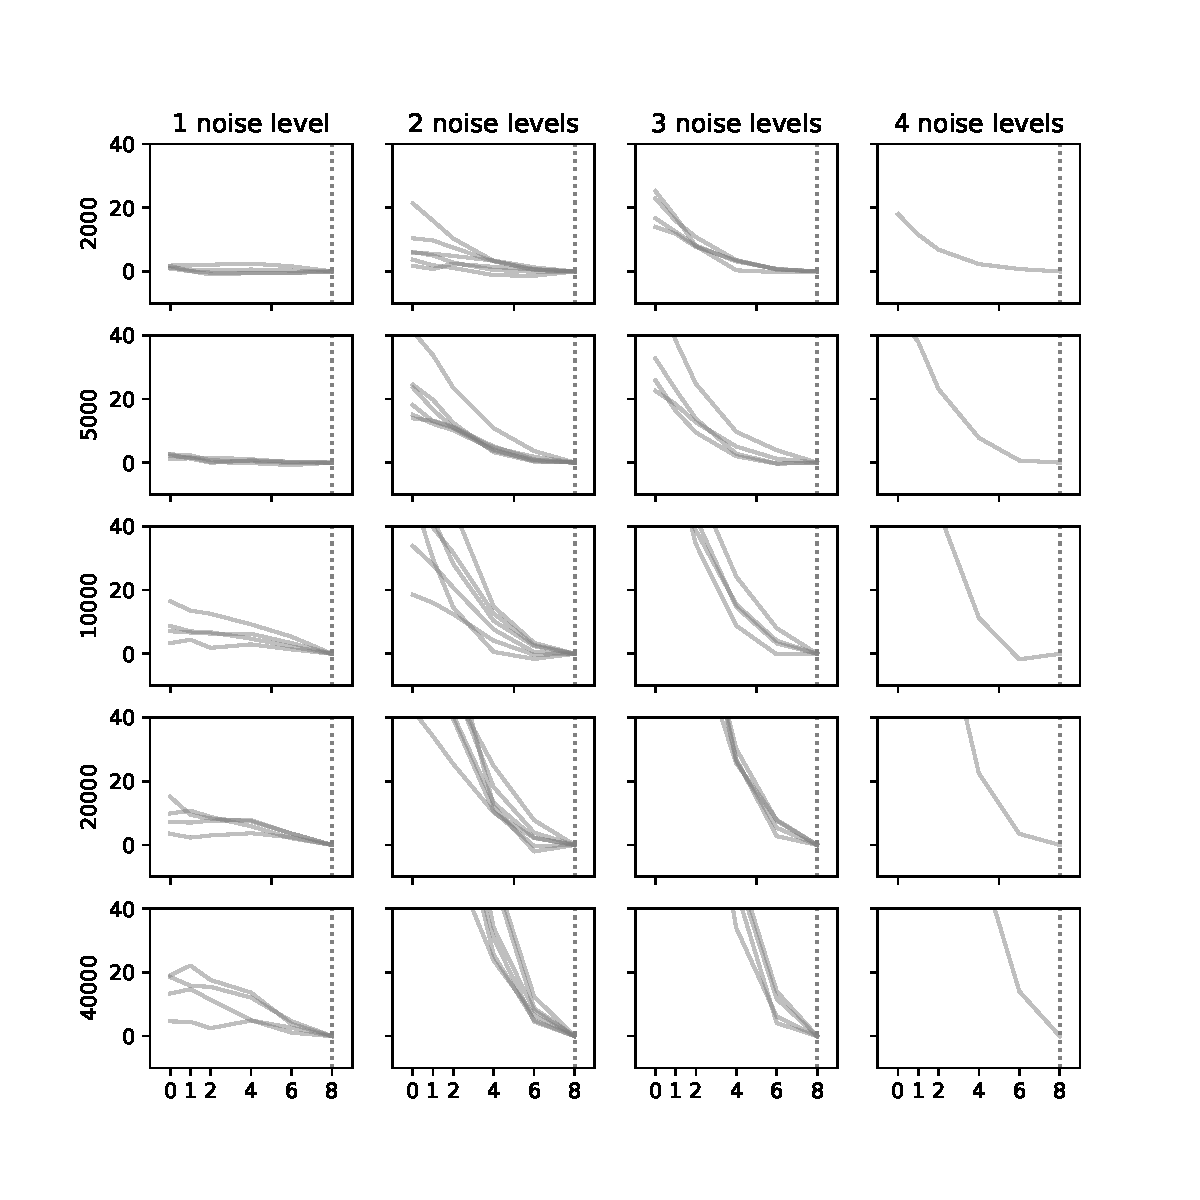
\includegraphics[width=0.33\textwidth]{figures/evaluateCrossValidationResults_Synthetic_Remington_VisualizeByNoiseCount_AndSize_ByP_Poster.py_UNIFORM_UNIMODAL2_8.pdf}
%%%%%%%
  \end{tabular}
\vspace{-4mm}
\caption{Interval Stimulus Space: Identifiability of the loss function depending on the number of trials and of sensory noise levels.}
\label{fig:uniform-unimodal}
\end{figure}


